 \section{Durchführung}
\label{sec:Durchführung}

\subsection{Vorbereitungsaufgabe}

Mit Formel \eqref{eqn:Dopplerwinkel} werden aus den Prismenwinkeln
\begin{align*}
  \theta_1 & = \SI{15}{\degree} \\
  \theta_2 & = \SI{30}{\degree} \\
  \theta_3 & = \SI{60}{\degree}
\end{align*}
die Dopplerwinkel
\begin{align*}
  \alpha_1 & = \SI{80.06}{\degree} \\
  \alpha_2 & = \SI{70.53}{\degree} \\
  \alpha_3 & = \SI{54.74}{\degree}
\end{align*}
bestimmt.

\subsection{Versuchaufbau}

Der Versuchsaufbau besteht aus einem Schlauchsystem, durch welches mit einer
Zentrifugalpumpe eine Dopplerphantomflüssigkeit, bestehend aus Wasser,
Glycerin und Glaskugeln, gepumpt wird.
Das Schlauchsystem ist ein Kreislauf mit drei verschiedenen Rohrdicken und
somit auch drei verschiedenen Strömungsgeschwindigkeiten. Mit der
Ultraschallsonde und mehreren Doppler-Prismen für die verschiedenen
Schlauchdurchmesser können mit Hilfe eines Ultraschall-Doppler-Generators
Schallfrequenzunterschiede und Intensitäten gemessen werden. Dabei muss darauf
geachtet werden, dass sich ausreichend Gel zwischen Sonde und Prisma und
Prisma und Schlauch befindet, damit die Schallwellen an den Grenzflächen
nicht bereits vollständig abgeschirmt werden, bevor sie die Flüssigkeit
erreichen. Mit einem
Computer werden die Daten aufgenommen und mit Hilfe des Programms
$FlowView$ analysiert, sodass die
Frequenzdifferenz abgelesen werden kann.
Bei der Analyse werden die Prismenwinkel mit der Formel
\begin{align}
  \alpha = \SI{90}{\degree} - \arcsin\Bigl(\sin{\theta}\frac{c_L}{c_P}\Bigr)
  \label{eqn:Dopplerwinkel}
\end{align}
umgerechnet, wobei $c_\text{L}$ die Schallgeschwindigkeit der Dopplerflüssigkeit
und $c_\text{P}$ die des Prismas (Acryl) ist.
Das Dopplerprisma ist in Abbildung \ref{fig:Dopplerprisma} dargestellt.

\begin{figure}
  \centering
  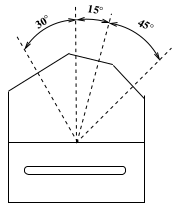
\includegraphics[height=4cm]{Dopplerprisma.png}
  \caption{Skizze des Dopplerprismas von der Seite. In diesem Versuch wird ein
  Dopplerprisma mit einem Winkel von $\SI{60}{\degree}$ statt $\SI{45}{\degree}$
  benutzt. \cite{anleitung}}
  \label{fig:Dopplerprisma}
\end{figure}

\subsection{Technische Daten}

Für den Versuchsaufbau sind folgende technische Daten gegeben:
\begin{align*}
  & \text{Dopplerphantomflüssigkeit:} \\
  & \text{Dichte} & \rho & = \SI{1.15}{\gram\per\cubic\centi\meter} \\
  & \text{Schallgeschwindigkeit} & c_\text{L} & = \SI{1800}{\meter\per\second} \\
  & \text{Viskosität} & \eta & = \SI{12}{\milli\pascal\second} \\ \\
  & \text{Dopplerprisma:} \\
  & \text{Schallgeschwindigkeit} & c_\text{P} & = \SI{2700}{\meter\per\second} \\
  & \text{Länge der Vorlaufstrecke} & l & = \SI{30.7}{\milli\meter} \\ \\
  & \text{Strömungsrohre:} \\
  & \text{Innendurchmesser} & l_\text{I} & = [7, 10, 16]\si{\milli\meter} \\
  & \text{Außendurchmesser} & l_\text{A} & = [10, 15, 20]\si{\milli\meter}
\end{align*}

\subsection{Messprogramm}

\subsubsection{Strömungsgeschwindigkeiten als Funktion des Dopplerwinkels}

\begin{enumerate}

  \item Zunächst wird das $Sample Volume$ an dem Ultraschallgenerator auf
  $Large$ gestellt.

  \item An einem beliebigen Schlauch werden jeweils fünf
  Frequenzdifferenzmesswerte bei verschiedenen
  Strömungsgeschwindigkeiten mit einer Pumpleistung von $\SI{40}{\percent}$ bis
  $\SI{70}{\percent}$ pro Winkel aufgenommen. Insgesamt werden also $15$
  Messwerte aufgenommen, da das Dopplerprisma drei Winkel besitzt.

  \item Die Messung wird an den anderen zwei Schläuchen wiederholt, sodass
  insgesamt weitere $30$ Messwerte hinzukommen.

\end{enumerate}

\subsubsection{Strömungsprofil der Dopplerflüssigkeit}

\begin{enumerate}

  \item Zunächst wird das $Sample Volume$ an dem Ultraschallgenerator auf
  $Small$ gestellt.

  \item Die Strömungsleistung an der Zentrifugalpumpe wird
  auf $\SI{70}{\percent}$ gestellt. Das Strömungsprofil wird nur an dem
  $\SI{10}{\milli\meter}$-Schlauch, bei einem Dopplerwinkel von
  $\SI{15}{\degree}$, gemessen.

  \item Mit dem Regler $Depth$ kann die Messtiefe am Ultraschallgenerator
  eingestellt werden. Es sollen nun für alle $32$ möglichen Tiefen, die
  eingestellt werden können, sowohl Streuintensität, als auch die
  Frequenzdifferenz aufgenommen werden.

  \item Diese Messung wird für eine Pumpleistung von $\SI{45}{\percent}$
  wiederholt.

\end{enumerate}
